\section{Our Approach}

Our approach is to break the stream up by time buckets and try various weak classifiers on buckets and then adjust our confidence over time.  The reason for using time based windows instead of a set amount of packets is that intuitively there is a better chance of identifying the application even if it is mixed with traffic from other applications on the tunnel. %(\ref{breakdown}).  
See \ref{windowclass} for classifying each time window and \ref{bayes} for information on updating the confidence over time.

%I am assuming that it reads better without the subsection. Feel free to revert.
%\subsection{Features}
We looked at two primary \emph{features} - packet size counts and timing between packets.  In our experience the timing was too noisy for accurate classification, but the packet size counts and relations between them are very useful.  And we can implicitly include some timing information by generating our feature vectors as a function of time.  So what we do is generate a single 65536 dimension feature vector where each dimension is a count of the number of packets with a size that is the same as the "number" of that dimension.

%\subsubsection{An example of where classifying a set amount of packets will break down}
%\label{breakdown}

As an illustration, if you take say 100 packets and treat that as your feature vector, and the user is 1) using skype and 2) watching a youtube video.  It is likely you will get no traffic for skype or at least not get consistent numbers of packets in that 100 length sequence due to being overwhelmed with video data.  On the other hand  in a 10 second window you can expect a certain amount of traffic from any particular application you are looking to identify, and our feature selection will ideally discard most of the noise.

Figure ~\ref{fig:bucket} displays a simple workflow with a 10 second window that saw 6 packets, 3 of which were sizes that the classifier deems relevant.

\begin{figure}
  \centering
  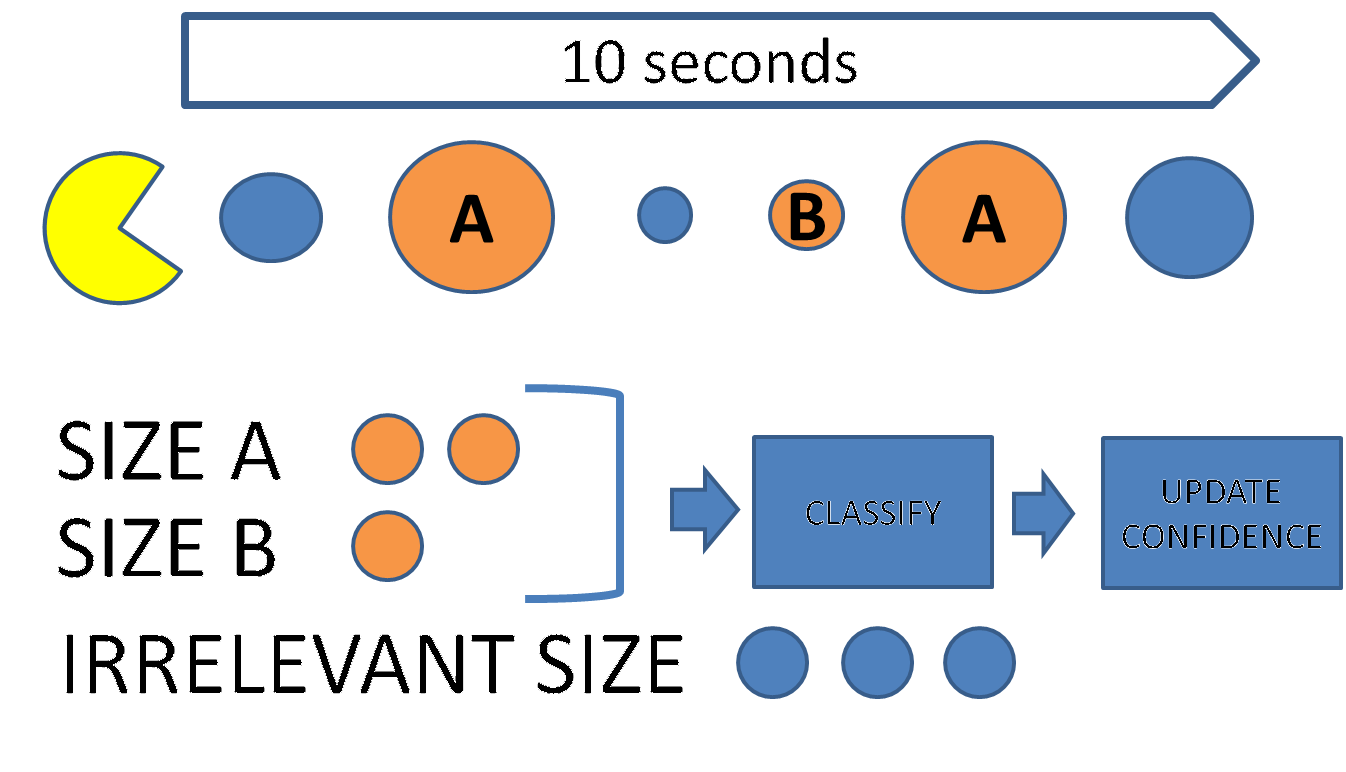
\includegraphics[width=0.9\textwidth]{bucketill.png}
  \caption{Illustration of bucketing sizes for a time window}
  \label{fig:bucket}
\end{figure}


\subsection{Algorithms used to classify 10 second windows of traffic}
\label{windowclass}

In order to be able to easily update our confidence using section ~\ref{bayes} our window classifier needs to return an estimate of the probability of the feature vector for both our negative and positive classes.  We should emphasize that
it is not  a probability that it belongs to the positive class.

\begin{description}

  \item[Likelihood function] Assume traffic is generated by a mixed gaussian and estimate the density function using the multi-variate normal likelihood function (Equation ~\eqref{eq:likelihood}).

  \item[Decision trees] See section ~\ref{dtree}.  This performs significantly better than the Likelihood function.

    \begin{flalign}
      \label{eq:likelihood}
      & L(\mathbf x) = e^{-\frac{1}{2} \ln(|\Sigma|) - \frac{1}{2}(\mathbf x - \mathbf \mu)^T \Sigma^{-1}(\mathbf x - \mathbf \mu) - \frac{k}{2} \ln(2 \pi)} & \\ \nonumber \\
      & \textbf{where} & \nonumber \\
      & \mathbf x = \text{column feature vector} & \nonumber \\
      & \mu = \text{Sample mean column vector} & \nonumber \\
      & \Sigma = \text{Sample covariance matrix} & \nonumber \\
      & |\Sigma| = \text{determinant of $\Sigma$} & \nonumber \\
      & k = \text{number of dimensions (65536)} & \nonumber
    \end{flalign}
\end{description}


\subsubsection{Decision Tree Algorithm}
\label{dtree}

\begin{figure}
  \centering
  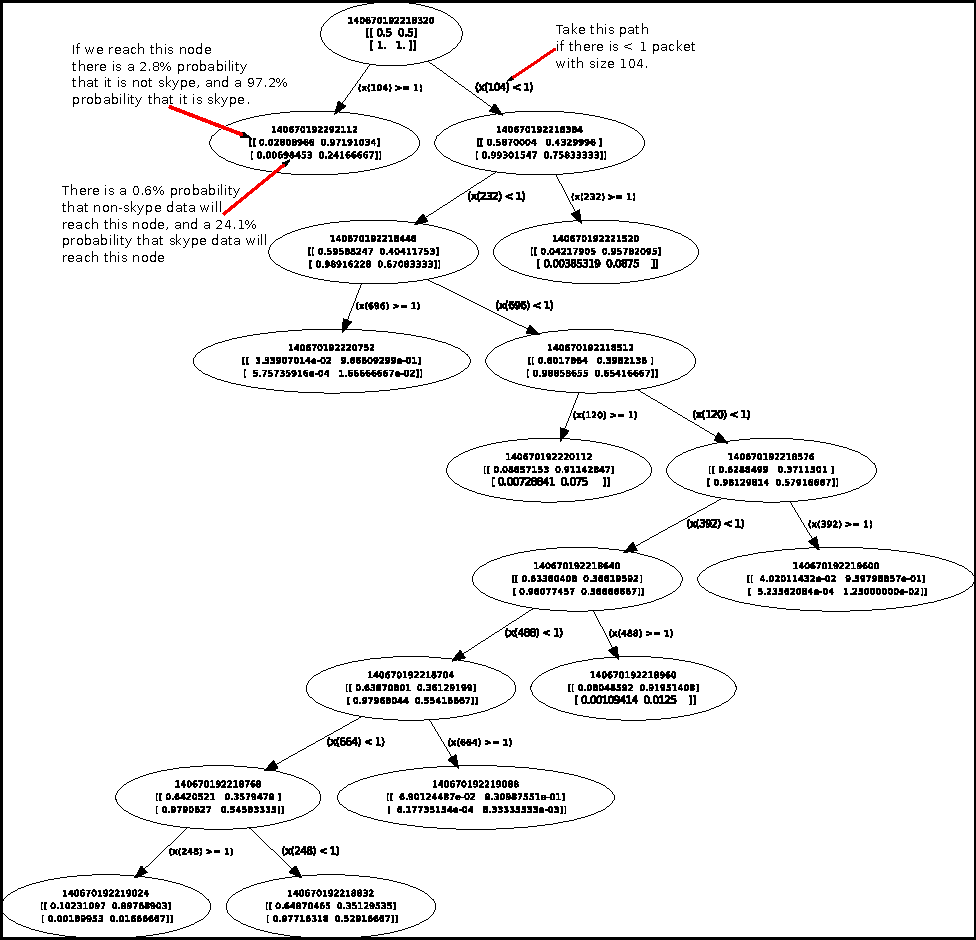
\includegraphics[width=0.9\textwidth]{sshdtree.pdf}
  \caption{Example Skype/SSH decision tree}
  \label{fig:dtree}
\end{figure}

See Figure ~\ref{fig:dtree} for an example of a Decision Tree that we would like to create.

Algorithm ~\ref{alg:dtree} describes the decision tree creation algorithm in pseudocode.  These trees give much better accuracy than the likelihood function and in fact get perfect accuracy with Skype, which most of the existing work has used.  The bias parameter is important to help avoid overfitting, and can be set by the user.  Additionally, the tools provided can search for the best bias.

\begin{algorithm}
  \caption{Decision Tree Creation Algorithm}
  \label{alg:dtree}
  \begin{algorithmic}
    \Function{SelectFeatureAndCutoff}{$data,bias$}
      \State $col \gets \bot$
      \State $cut \gets \bot$
      \State $max \gets -\infty$

      \ForAll{$\{column,thresh | column,thresh \in features \times values\}$}
        \State $igain \gets \text{information gain ratio using column and thresh}$
        \\\\
        \Comment{We use the $bias$ parameter to bias our selection to column/thresh pairs that look for a decrease in the probability of the positive class on the $<$ side, this is so that we do not learn that a protocol "will not have these sizes"}
        \\\\

        \State $score \gets {(P(col >= thresh | positive) * \frac{P(col >= thresh | positive)}{P(col >= thresh | negative)} * igain^{bias})}^\frac{1}{2 + bias}$
        \If{$score > max$}
          \State $max \gets score$
          \State $col \gets column$
          \State $cut \gets thresh$
        \EndIf
      \EndFor

      \State \Return $col, cut$
    \EndFunction
    \\\\
    \Function{ExpandNode}{$data,bias$}
      \State $p \gets \text{probability of positive class given } data$
      \If{$p < \epsilon \lor p > 1 - \epsilon$}
        \State \Return
      \EndIf
      \State $f,c \gets \text{SelectFeatureAndCutoff(}data,bias\text{)}$
      \State $low \gets \{ x | x \in data \land x[f] < c \}$
      \State $high \gets \{ x | x \in data \land x[f] >= c \}$
      \State ExpandNode($low$)
      \State ExpandNode($high$)
    \EndFunction
    \\\\
    ExpandNode(training data)
  \end{algorithmic}
\end{algorithm}

\subsection{Using Bayes Rule to update our confidence}
\label{bayes}

\paragraph
For each network stream we maintain a probability that the stream contains data from our positive class ($P(CLASS|DATA)$).  For every 10 seconds of data we then create a feature vector and estimate $P(DATA|CLASS)$ for both the positive and negative classes using either the likelihood function or decision trees.  Once we have this estimate we can update our stored prior (confidence if you prefer) using Bayes' Rule (Equation \eqref{eq:bayes}).

\begin{equation}
  \label{eq:bayes}
  P(CLASS|DATA) = \frac{P(DATA|CLASS) P(CLASS)}{\Sigma_{C \in CLASSES}{P(DATA|C) P(C)}}
\end{equation}
